% --------------------------------------------------
% 1. INTRODUCTION
% --------------------------------------------------
\section{Introduction}

In May 2013, Bradley Wiggins, the reigning Tour de France champion, abandoned the Giro d'Italia after just seven stages. His departure was not simply a sporting story. Team Sky had built its entire Giro campaign around Wiggins, allocating domestiques, logistics, and media attention to support his General Classification (GC) bid. When he climbed off his bike, the team lost its primary investment for the race, sponsors lost three weeks of planned television exposure, and Wiggins himself saw his market value as a Grand Tour rider come under scrutiny. Episodes like this raise a question at the intersection of sports and economics: what determines whether a rider continues or abandons a Grand Tour?

This paper treats rider abandonment as an economic decision. At every stage of a Grand Tour, the rider and his team face a choice under uncertainty: continue and bear the physical and strategic costs, or withdraw and reallocate effort toward future races. This framing connects to tournament theory \parencite{rosen1981superstars, lazear1981rank}, where the structure of rewards creates position-dependent incentives, and to the sports-labour-market literature \parencite{kahn2000labormarket}, where observable performance signals affect a rider's future contract value. The course textbook \parencite{blair2012sports} provides the broader framework for understanding professional sports organisations as economic actors operating under these forces.

The research question is: 
\emph{How do proxy measures of economic incentives and continuation costs explain rider abandonment in Grand Tours?} The word ``proxy'' 
is important. The dataset does not contain direct financial variables such as prize money, rider salaries, or team budgets. Instead, the analysis uses observable covariates that can be interpreted as reflecting underlying economic forces: whether a rider is classified as a GC contender proxies for expected returns, while a rider's historical abandonment rate captures information about expected continuation costs.

To answer this question, the paper draws on a self-constructed panel dataset of 9{,}045 rider-race observations covering all three Grand Tours (the Tour de France, Giro d'Italia, and Vuelta a Espa\~{n}a) from 2010 to 2025, scraped from ProCyclingStats. As Figure~\ref{fig:dnf_by_year} illustrates, abandonment rates vary across races and over time, with the Tour de France consistently showing the lowest rates. This variation motivates the empirical investigation: if abandonment were purely random or driven only by physical factors, we would not expect such persistent differences.

\begin{figure}[H]
    \centering
    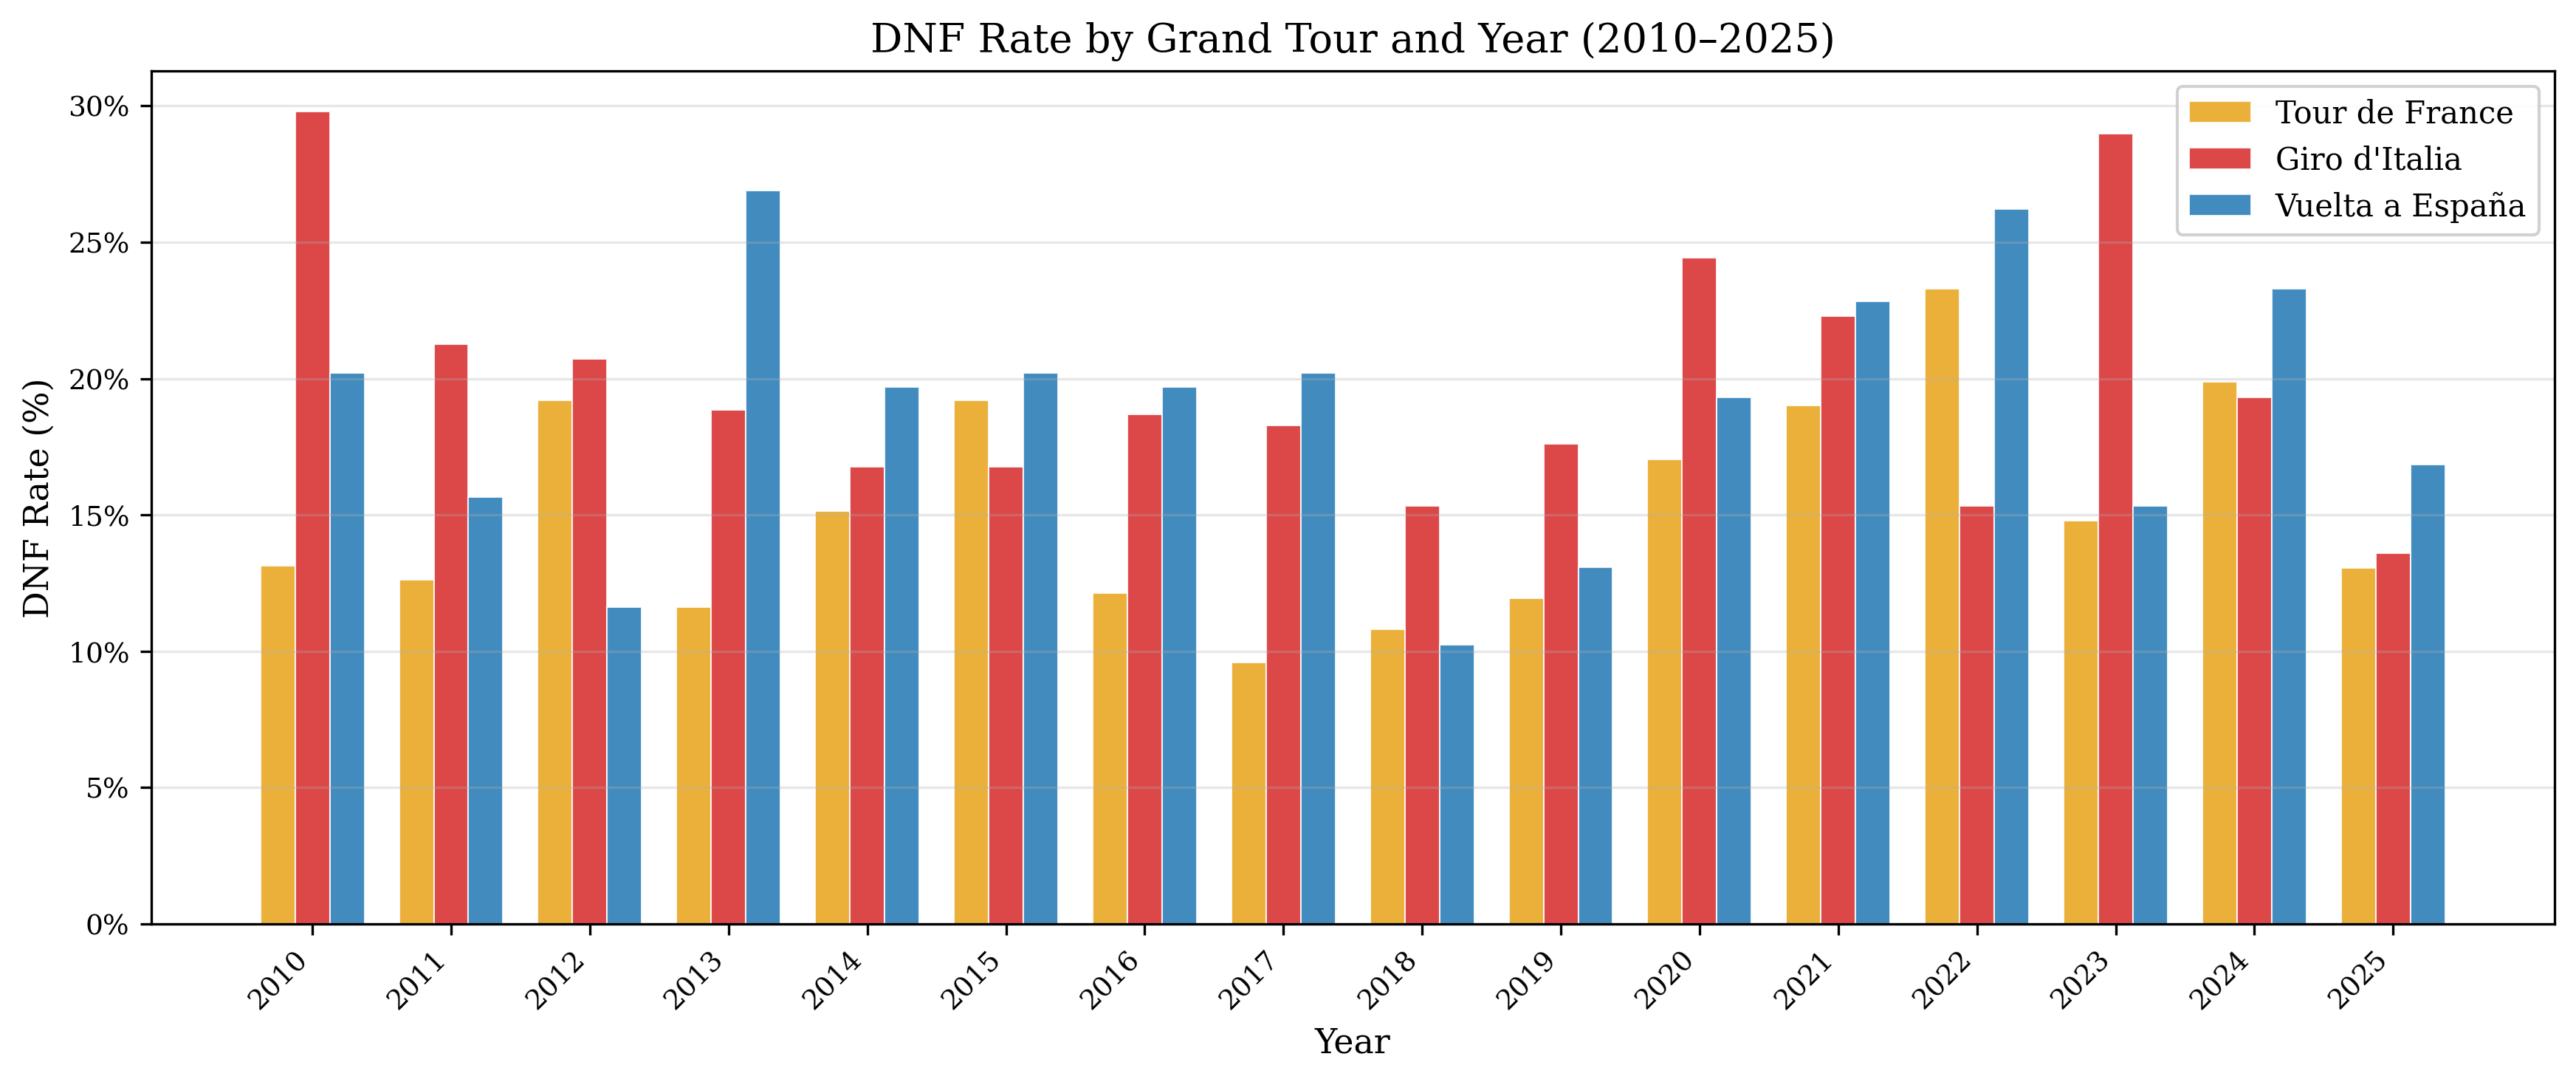
\includegraphics[width=0.5\linewidth]{Afsnit/Billeder/fig2_dnf_rate_by_race_year.png}
    \caption{DNF rate by Grand Tour and year (2010--2025). The Tour de France consistently shows the lowest abandonment rate, while the Giro d'Italia typically shows the highest.}
    \label{fig:dnf_by_year}
\end{figure}

The econometric approach uses Cox proportional hazard models, which model the instantaneous probability of abandonment at each stage conditional on the rider still being in the race. A time-varying extension adds stage-level covariates that change from stage to stage within a race. The main findings are: (i) a rider's historical DNF rate is the strongest predictor of abandonment (HR $= 1.55$, $p < 0.001$); (ii) the Tour de France has significantly lower abandonment hazard than the Vuelta (HR $= 0.865$, $p = 0.002$); and (iii) mountain stages raise daily abandonment hazard (HR $= 1.034$, $p = 0.025$).

The paper is structured as follows. Section~\ref{sec:theory} presents the theoretical framework and reviews relevant literature. Section~\ref{sec:data} describes the data and variables. Section~\ref{sec:empirical_strategy} explains the methodology. Section~\ref{sec:results} presents results. Section~\ref{sec:robustness} provides robustness checks. Section~\ref{sec:discussion} discusses the economic and managerial implications of the findings. Section~\ref{sec:conclusion} concludes with limitations and suggestions for future research.
